% \documentclass[12pt, twoside]{article}
\usepackage[letterpaper, margin=1in, headsep=0.2in]{geometry}
\setlength{\headheight}{0.6in}
%\usepackage[english]{babel}
\usepackage[utf8]{inputenc}
\usepackage{microtype}
\usepackage{amsmath}
\usepackage{amssymb}
%\usepackage{amsfonts}
\usepackage[nomessages]{fp} %\FPeval{\var-name}{2*sin(pi/6)}
\usepackage{siunitx} %units in math. eg 20\milli\meter
\usepackage{yhmath} % for arcs, overparenth command
\usepackage{tikz} %graphics
\usetikzlibrary{quotes, angles, arrows, arrows.meta}
\usepackage{graphicx} %consider setting \graphicspath{{images/}}
\usepackage{parskip} %no paragraph indent
\usepackage{enumitem}
\usepackage{multicol}
\usepackage{venndiagram}

\usepackage{fancyhdr}
\pagestyle{fancy}
\fancyhf{}
\renewcommand{\headrulewidth}{0pt} % disable the underline of the header
\raggedbottom
\hfuzz=2mm %suppresses overfull box warnings

\usepackage{hyperref}

\fancyhead[LE]{\thepage}
\fancyhead[RO]{\thepage \\ Name: \hspace{4cm} \,\\}
\fancyhead[LO]{BECA / Dr. Huson / Geometry\\*  Unit 11: Circle angles, sectors, arcs \\* 27 February 2023}

\begin{document}

\subsubsection*{11.1 Homework: Circle arcs, sectors, central angles}
\begin{enumerate}
  \item Given circle $O$ with various internal line segments as shown.
  \begin{multicols}{2}
  \raggedcolumns
  \begin{enumerate}[itemsep=0.5cm]
    \item Highlight each radius in red
    \item Highlight any chords in yellow
    \item Is the $\angle CAD$ an inscribed angle or a central angle?
    \item Is $\triangle AOB$ an equilateral triangle, isosceles triangle, or a scalene triangle?
  \end{enumerate}
  \begin{tikzpicture}[scale=0.7]
    \draw (0,0) circle[radius=4];
    \draw [thick]
    (-4,0) node[left] {$A$}--
    (0,0) node[below] {$O$}--
    (4,0) node[below left] {$C$};
    \draw [thick]
    (0,0) -- (50:4) node[above right] {$B$}--(-4,0);
    \draw [thick]
    (-4, 0)--
    (-100:4) node[below] {$D$};
    \node at (0,0) {$\bullet$};
  \end{tikzpicture}
  \end{multicols}

\item Given circle $O$ with points on the circle $A$, $B$, $C$, $D$ as shown. Find each central angle measure.
\begin{multicols}{2}
  \begin{enumerate} 
    \item $m\angle AOB =$
    \item $m\angle BOC =$
    \item $m\angle AOC =$
    \item What is the measure of the \emph{reflex angle} $m\angle AOC =$, i.e. the one containing point $D$ that is $>180^\circ$
    \end{enumerate}
    \begin{tikzpicture}[scale=0.8]
      \draw (0,0) circle[radius=4];
      \draw [thick]
      (-80:4) node[below left] {$B$}--
      (0,0) node[above] {$O$}--
      (-160:4) node[below left] {$A$};
      \draw [thick]
      (0,0) -- (-20:4) node[right] {$C$};
      %\node at (0,0) {$\bullet$};
      \fill (0,0) circle[radius=.1];
      \fill (70:4) circle[radius=.1]node[above]{$D$};
      \node at (-50:1.25) {$60^\circ$};
      \node at (-115:1.2) {$70^\circ$};
    \end{tikzpicture}
\end{multicols}

\item Lesson: Any portion of the circumference of a circle is called an \emph{arc} and written $\wideparen{AB}$. \\[0.25cm]
A \emph{sector} is part of a circle (``pie slice'') bounded by two radii and an arc.
  \begin{multicols}{2}
  \raggedcolumns
  \begin{enumerate}[itemsep=0.5cm]
    \item Highlight arc $\wideparen{AB}$.
    \item An arc's degree measure equals its corresponding central angle measure. \\[0.25cm]
    If $m\angle AOB = 60^\circ$, what is the $m \wideparen{AB}$?
    \item A \emph{semicircle} is half of a circle.
    \item An arc smaller than half a circle is a \emph{minor} arc, one larger is a \emph{major} arc. \\[0.25cm]
    Which is a major arc, $\wideparen{AB}$ or $\wideparen{ACB}$?
  \end{enumerate}
  \begin{tikzpicture}[scale=0.8]
    \draw (0,0) circle[radius=4];
    \draw [thick]
    (0:4) node[right] {$A$}--
    (0,0) node[left] {$O$}--
    (60:4) node[above right] {$B$};
    \fill (130:4) circle[radius=.1]node[above]{$C$};
    \fill (0,0) circle[radius=.1];
    \node at (30:1.25) {$60^\circ$};
  \end{tikzpicture}
  \end{multicols}

\item A regular hexagon is inscribed in a circle with a radius $r=12$, as shown.
  \begin{multicols}{2}
  \raggedcolumns
  \begin{enumerate}[itemsep=2cm]
    \item Find the circumference of the circle in terms of $\pi$. ($C=2\pi r$)
    \item How long is the curved part of the circle from point $A$ to $B$, $\wideparen{AB}$?
    \item What is the degree measure of the arc from point $A$ to $C$,  $m \wideparen{AC}$?
  \end{enumerate}
  \begin{tikzpicture}[scale=0.8]
    \draw (0,0) circle[radius=4];
    \draw [thick, dotted]
    (0:4) node[above right] {$A$}--
    (0,0) node[left] {$O$}--
    (60:4) node[above right] {$B$};
    \draw [thick]
    (0:4) -- (60:4)-- (120:4)-- (180:4)-- (240:4)-- (300:4)-- cycle;
    \fill (120:4) circle[radius=.1]node[above]{$C$};
    \fill (0,0) circle[radius=.1];
    \node at (30:1.25) {$60^\circ$};
    \node at (-10:2.25) {$12$};
  \end{tikzpicture}
  \end{multicols}

\item A regular pentagon is inscribed in a circle with a radius $r=10$, as shown.
  \begin{multicols}{2}
  \raggedcolumns
  \begin{enumerate}[itemsep=2cm]
    \item Find the circle's area in terms of $\pi$. ($A=\pi r^2$)
    \item What is the degree measure of the central angle $\angle AOB$?
    \item What is the area of the sector bounded by $\overline {AO}$, $\overline {BO}$, and $\wideparen{AB}$?
  \end{enumerate}
  \begin{tikzpicture}[scale=0.8]
    \fill [lightgray]
    (0,0)--(0:4) arc (0:72:4)--(0,0);
    \draw (0,0) circle[radius=4];
    \draw [thick, dotted]
    (0:4) node[above right] {$A$}--
    (0,0) node[left] {$O$}--
    (72:4) node[above right] {$B$};
    \draw [thick]
    (0:4) -- (72:4)-- (144:4)-- (216:4)-- (288:4)--cycle;
    \fill (0,0) circle[radius=.1];
    \node at (35:1) {$?$};
    \node at (-10:2.25) {$10$};
  \end{tikzpicture}
  \end{multicols}


\end{enumerate}
\end{document}
